\documentclass{jarticle}
\usepackage{rsj}
\usepackage[dvips]{graphicx}
\usepackage{url}
\usepackage{bm}
\usepackage{amsmath}
\usepackage{amssymb}
\newcommand*{\Scale}[2][4]{\scalebox{#1}{$#2$}}%

\begin{document}
\title{Motion Primitive with Aerial Manipulator for Dynamic Tennis Swing Motion}
\author{Fan Shi\ \ Moju Zhao\ \ Tomoki Anzai\ \ Xiangyu Chen\ \ Kei Okada\ \ Masayuki Inaba}

\setlength{\baselineskip}{4.4mm}
\maketitle
\thispagestyle{empty}
\pagestyle{empty}

\section{Introduction}

In this paper, we implement a rapid real-time motion planning algorithm with a novel type of aerial manipulator, and dynamic tennis swing motion is achieved as an example to show the feasibility of the algorithm. When planning the feasible trajectory, dynamic constraints of the robot, and position, velocity and acceleration in start and end points are considered. Thousands of motion primitives are generated online and the least-cost trajectory to follow is selected by trajectory selector.

Recently, aerial robots raise increasing attentions and lots of fundamental researches appear in geometric control, 3D mapping,  and real-time planning. With the help of these fundamental researches, aerial robots shows great potential to interact with environments and take more complex tasks such as multi-field drone, moving collaborate object. Among them, aerial manipulator is the most exciting and difficult one since it directly interact with the environments. Several researches of aerial manipulators are shown, some work attaches a high-DOFs robot arm to the downward base of the drone and more consideration in stability and workspace is needed\cite{aerial_manipulator_1}, some are a simple 1-DOF gripper with limited functions\cite{aerial_manipulator_2}. Hence, our lab come up with a transformable drone (Hydrus \reffig{abst-image}) as the aerial manipulator with dual arms, which have lots of potentials like moving in clustered environments and moving heavy objects\cite{zhao_ar}\cite{zhao_iser}.

In the following sections, we will design motion planning framework for Hydrus robot and use experiment result to verify the feasibility.

\begin{figure}[htb]
  \centering
  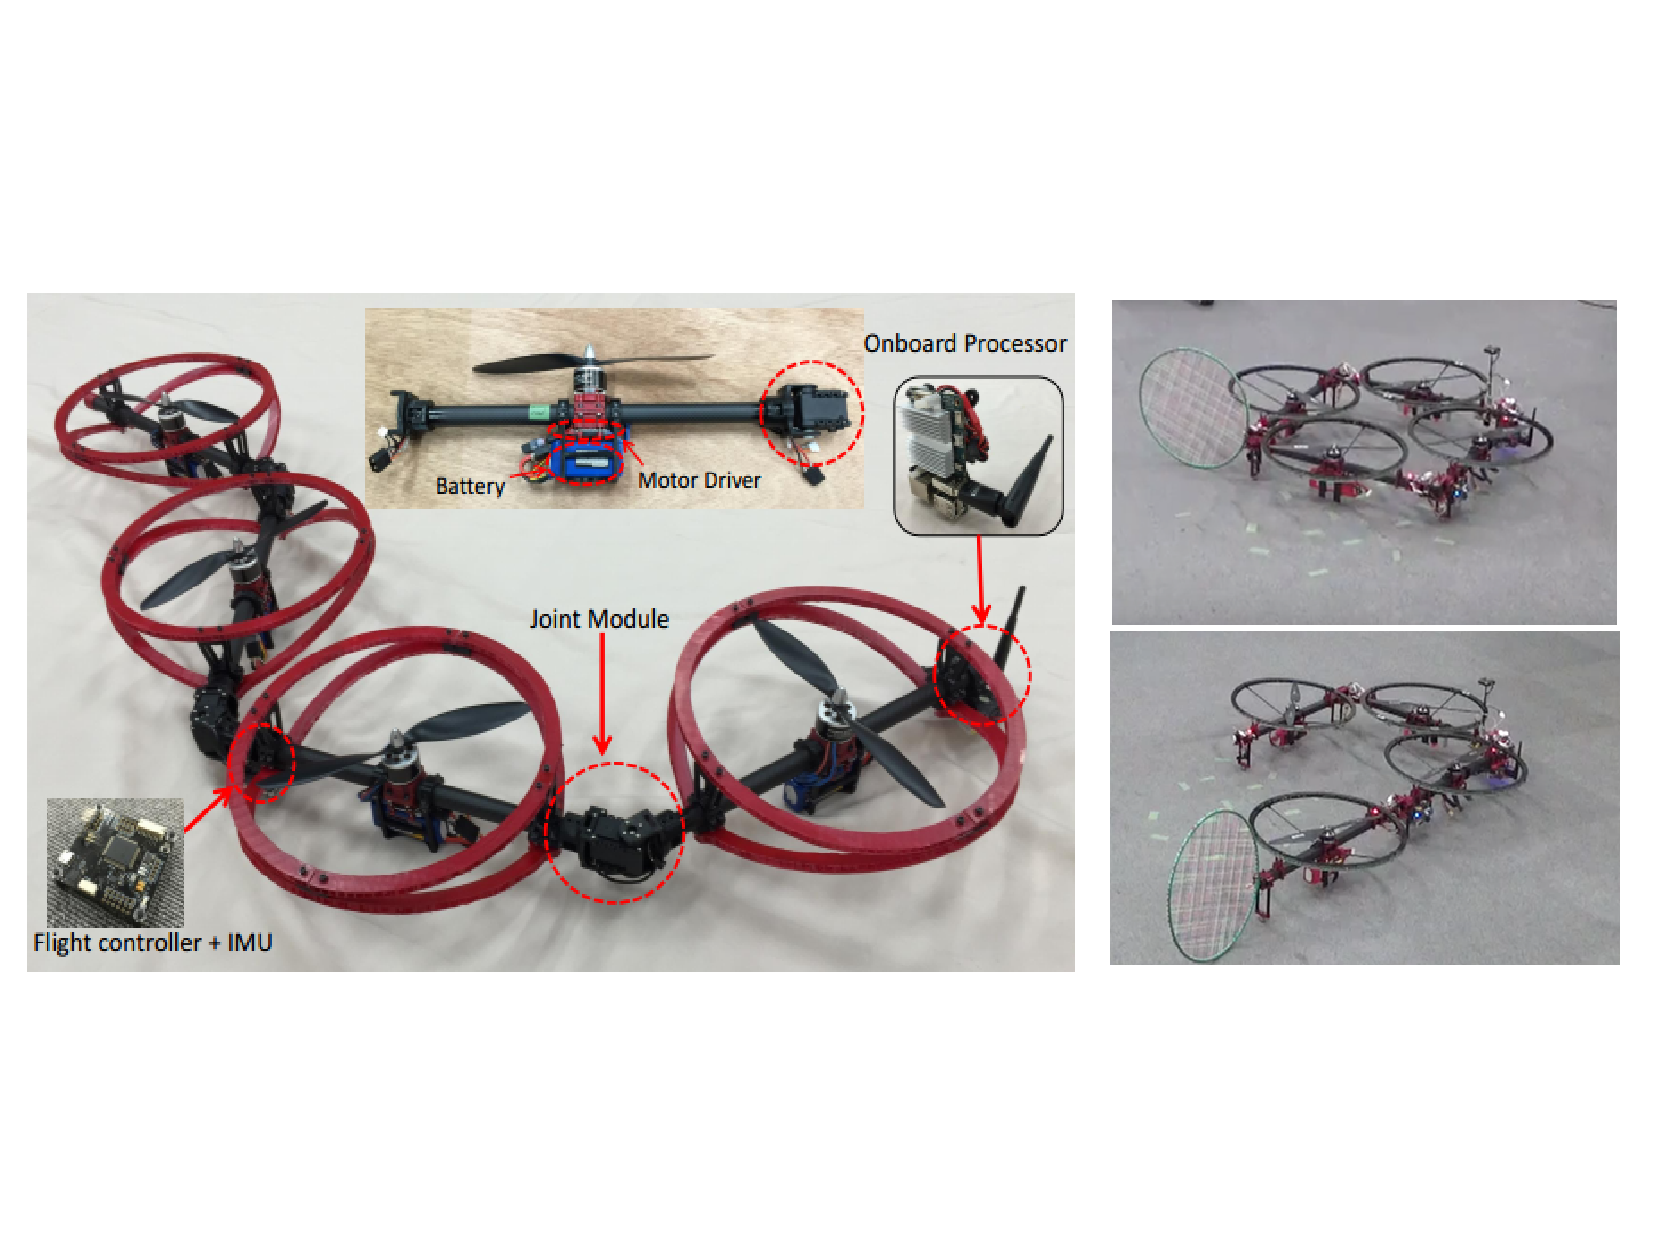
\includegraphics[clip, bb= 10 128 777 457,  width=\columnwidth]{figs_orig/figure.pdf}
  \caption{Left is the basic structure of 4-links Hydrus robot, which has 4 rotors and 3 motor-driven joint links. Right is Hydrus robot with tennis racket.}
  \label{fig:abst-image}
\end{figure}

\section{Dynamic Tennis Swing Motion}

\subsection{Model}
Geometric control researches showed the differential flatness of quadrotor  system[1], which means that the output of 4 rotors rotation speed could be calculated based on the given input [x, y, z, ψ], here x, y, z, ψ is the function x(t), y(t), z(t), ψ(t)  representing the position of robot in x, y, z axis and yaw angle at time t.
The dynamics of the translational motion and rotation motion can be described as follows:
\begin{equation}
  \label{eq:model1}
  M^{\scalebox{.5}{$\{W\}$}}\bm{\ddot{r}}_{CoG} =\left[ \begin{array}{c}
      0 \\
      0 \\
      -M^{\scalebox{.5}{$\{w\}$}}g
    \end{array}\right]
  + {}^{\scalebox{.5}{$\{W\}$}}R \left[ \begin{array}{c}
        0 \\
        0 \\
        \sum_{i=1}^{N} {}^{\scalebox{.5}{$\{CoG\}$}}F_i
      \end{array}\right]
\end{equation}

\begin{eqnarray}
  \label{eq:model2-0}
  & {}^{\scalebox{.5}{$\{CoG\}$}}I_{multilink} \left[ \begin{array}{c}
      {}^{\scalebox{.5}{$\{CoG\}$}}\dot{w} _x \\
      {}^{\scalebox{.5}{$\{CoG\}$}}\dot{w} _y \\
      {}^{\scalebox{.5}{$\{CoG\}$}}\dot{w} _z
    \end{array}\right]
  = \left[ \begin{array}{c}
      \sum_{i=1}^{N} {}^{\scalebox{.5}{$\{CoG\}$}}y_i {}^{\scalebox{.5}{$\{CoG\}$}}F_i \\
      -\sum_{i=1}^{N} {}^{\scalebox{.5}{$\{CoG\}$}}x_i {}^{\scalebox{.5}{$\{CoG\}$}}F_i \\
      \sum_{i=1}^{N} {}^{\scalebox{.5}{$\{CoG\}$}}T_i
    \end{array}\right] \nonumber \\
  \label{eq:model2}
  & - \left[ \begin{array}{c}
      {}^{\scalebox{.5}{$\{CoG\}$}}w_x \\
      {}^{\scalebox{.5}{$\{CoG\}$}}w_y \\
      {}^{\scalebox{.5}{$\{CoG\}$}}w_z
    \end{array}\right]
  \times {}^{\scalebox{.5}{$\{CoG\}$}}I_{multilink} \left[ \begin{array}{c}
      {}^{\scalebox{.5}{$\{CoG\}$}}w_x \\
      {}^{\scalebox{.5}{$\{CoG\}$}}w_y \\
      {}^{\scalebox{.5}{$\{CoG\}$}}w_z
    \end{array}\right]
\end{eqnarray}

%% \begin{equation}
%%   \label{eq:model2}
%% %%   I_{multilink} \left[ \begin{array}{c}
%% %%       \dot{w} _x \\
%% %%       \dot{w} _y \\
%% %%       \dot{w} _z
%% %%     \end{array}\right]
%% %%   = \left[ \begin{array}{c}
%% %%       \sum_{i=1}^{N} y_i  \\
%% %%       \sum_{i=1}^{N}  \\
%% %%       \sum_{i=1}^{N} T_i
%% %%     \end{array}\right]
  
%% \end{equation}




\subsection{Motion Primitive}
In robotic trajectory planning researches, optimization and sampling based methods are two mainstreams. Optimization based methods is usually time consuming, so in this paper we develop a rapid motion primitive algorithm based on sampling methods.

We develop a motion primitive method based on differential flatness quality, and 6-order polynomial functions are calculated in every axis and keep yaw angle to be fixed in the whole trajectory. Then jerk will be evaluated as the smoothness of the trajectory\cite{eth-juggling}.

The motion primitive in each axis follows:

\begin{equation}
  \label{eq:temp}
  \bm{f}(t) = \left[ \begin{array}{c}
      \bm{x}(t) \\
      \bm{v}(t) \\
      \bm{a}(t)
    \end{array}\right]
\end{equation}

\begin{equation}
  \label{eq:temp2}
  \bm{f}(t) = \begin{bmatrix}
      \bm{a} & \bm{b} & \bm{c} & \bm{d} & \bm{e} & \bm{f} \\
      0 & 5\bm{a} & 4\bm{b} & \bm{c} & 2\bm{d} & \bm{e} \\
      0 & 0 & 20\bm{a} & 12\bm{b} & 6\bm{c} & 2\bm{d}
  \end{bmatrix}
  *
  \left[ \begin{array}{c}
      1 \\
      t \\
      t^2 \\
      t^3 \\
      t^4 \\
      t^5
    \end{array}\right]
\end{equation}


For any random start point, we could acquire its position, velocity and acceleration from robot inertial data. The end point would be the hitting point, and its position, velocity and acceleration could be sampled in the work space. Considering a simple situation, we assume tennis ball is fixed, so only velocity and acceleration are needed to be sampled. For traverse time, we use traverse trajectory distance and average traverse speed to get the traverse time.

To get the faster swing speed, motion primitive for swing joint is also generated(\reffig{primitive-image}). The racket attached joint will backswing in advance, and then swing to guarantee racket will have velocity when being in collision with tennis ball. The backswing and swing time is decided by the selected trajectory of the robot.

\subsection{Trajectory Selection}
Considering the dynamic feasibility of the robot, the maximum velocity and acceleration have to be guaranteed. So the selector is as:

\begin{eqnarray}
  \label{eq:temp3}
 & min{\int_0^T |f^{(3)}_x(t) + f^{(3)}_y(t) + f^{(3)}_z(t)|^2 dt}   \\
  \label{eq:temp4}
s.t. &  V_{i_{min}} < f^{(1)}_i(t) < V_{i_{max}}, i = x, y, z \nonumber \\
  \label{eq:temp5}
 & a_{i_{min}} < f^{(2)}_i(t) < a_{i_{max}}, i = x, y, z \nonumber \\
  \label{eq:temp6}
 & 0 < f_z(t) \nonumber
\end{eqnarray}

Objective function is showed as \refeq{temp3}, the calculus of the jerk’s absolute value from start time to end time is calculated. The following constraints guarantee the dynamic constraints of robot and robot not crashing into the ground.

If there are other obstacles except for the ground in the environment, collision-free constraints should be considered as:

\begin{equation}
  \label{eq:temp7}
  C_{obstacle}\bigcap (f_x(t), f_y(t), f_z(t)) =\emptyset
\end{equation}


\begin{figure}[htb]
  \centering
  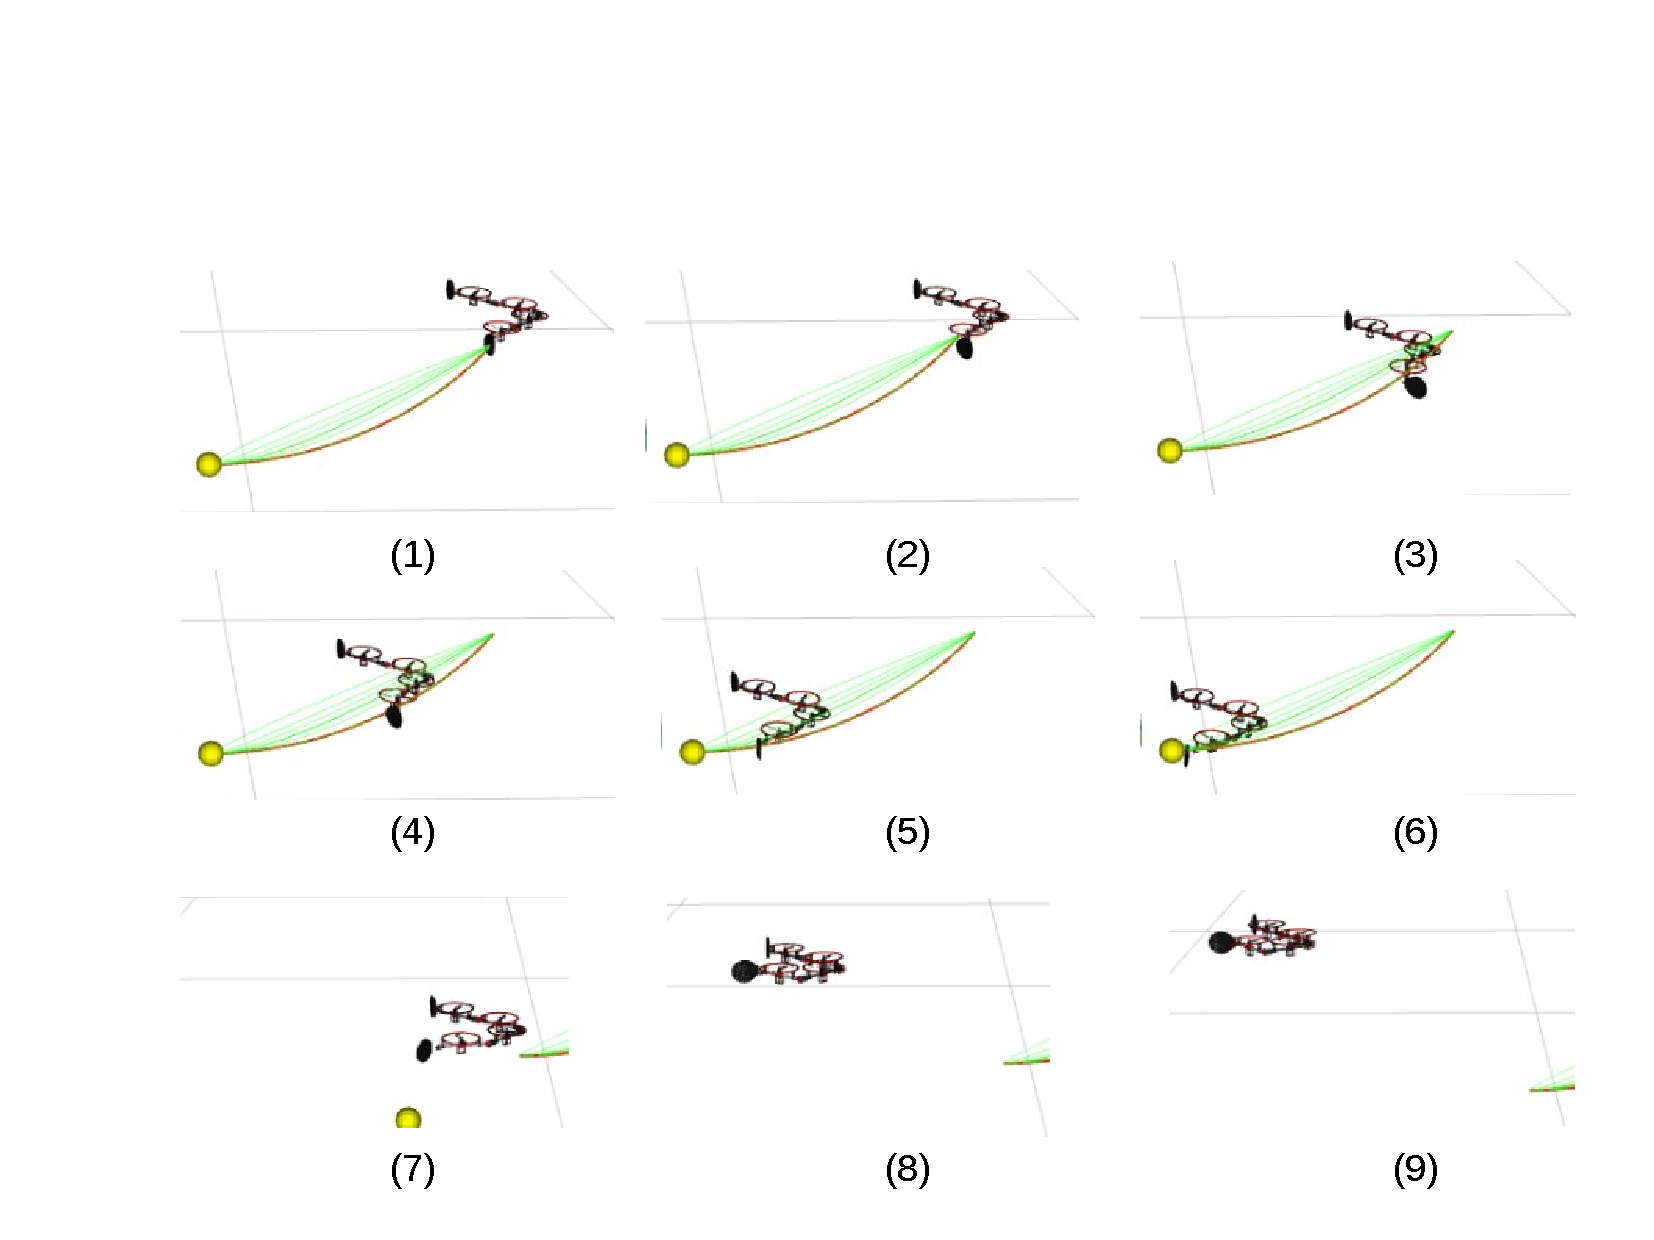
\includegraphics[clip, bb= 61 16 770 488,  width=\columnwidth]{figs_orig/primitive.pdf}
  \caption{(1)-(6) is the swing motion based on motion primitive, green lines are primitive candidates, red line is the selected candidate, yellow ball is the hitting target. (1) is the start point, (2) begins to do backswing, (3) finishes backswing, (4) starts swing motion, (5) gets close to target and continue swing motion, (6) hits the target ball.\newline (7)-(9) is the attitude control after hitting motion, robot recovers to be still and specific height. }
  \label{fig:primitive-image}
\end{figure}

\section{Simulation Result}
We implement this method into Gazebo simulation and nearly 5, 000 motion primitives could be generated in 100ms, and feasible trajectory could be easily found inside these candidates \reffig{primitives}. Then we build position and velocity control loop to guarantee the robot could follow the feasible trajectory.

\section{Conclusion}
This paper showed a rapid motion planning algorithm for Hydrus robot, and implement tennis swing task as the example to show the feasibility of the method. Experiment is implemented in simulation and the whole system is evaluated.

For future work, we are expecting to implement the method into real physical Hydrus robot to evaluate the whole system. And the use of GPU to accelerate motion primitive calculation is also considered. Perception of the tennis ball to generate catch-and-swing motion will be implemented as the future work.

{\footnotesize
%\small
\bibliographystyle{junsrt}
\bibliography{main}
}
\end{document}
